\documentclass[thesis.tex]{subfiles}

\title{Estimating duration in the presence of misclassification}
\author{Joshua Blake}
\date{\today}

\begin{document}

\ifSubfilesClassLoaded{
  \setcounter{chapter}{1}
}

\chapter{SARS-CoV-2: biology and data} \label{intro:sec:studies}

\section{Natural history of the disease} \label{biology-data:sec:natural-history}

\begin{figure}
  \centering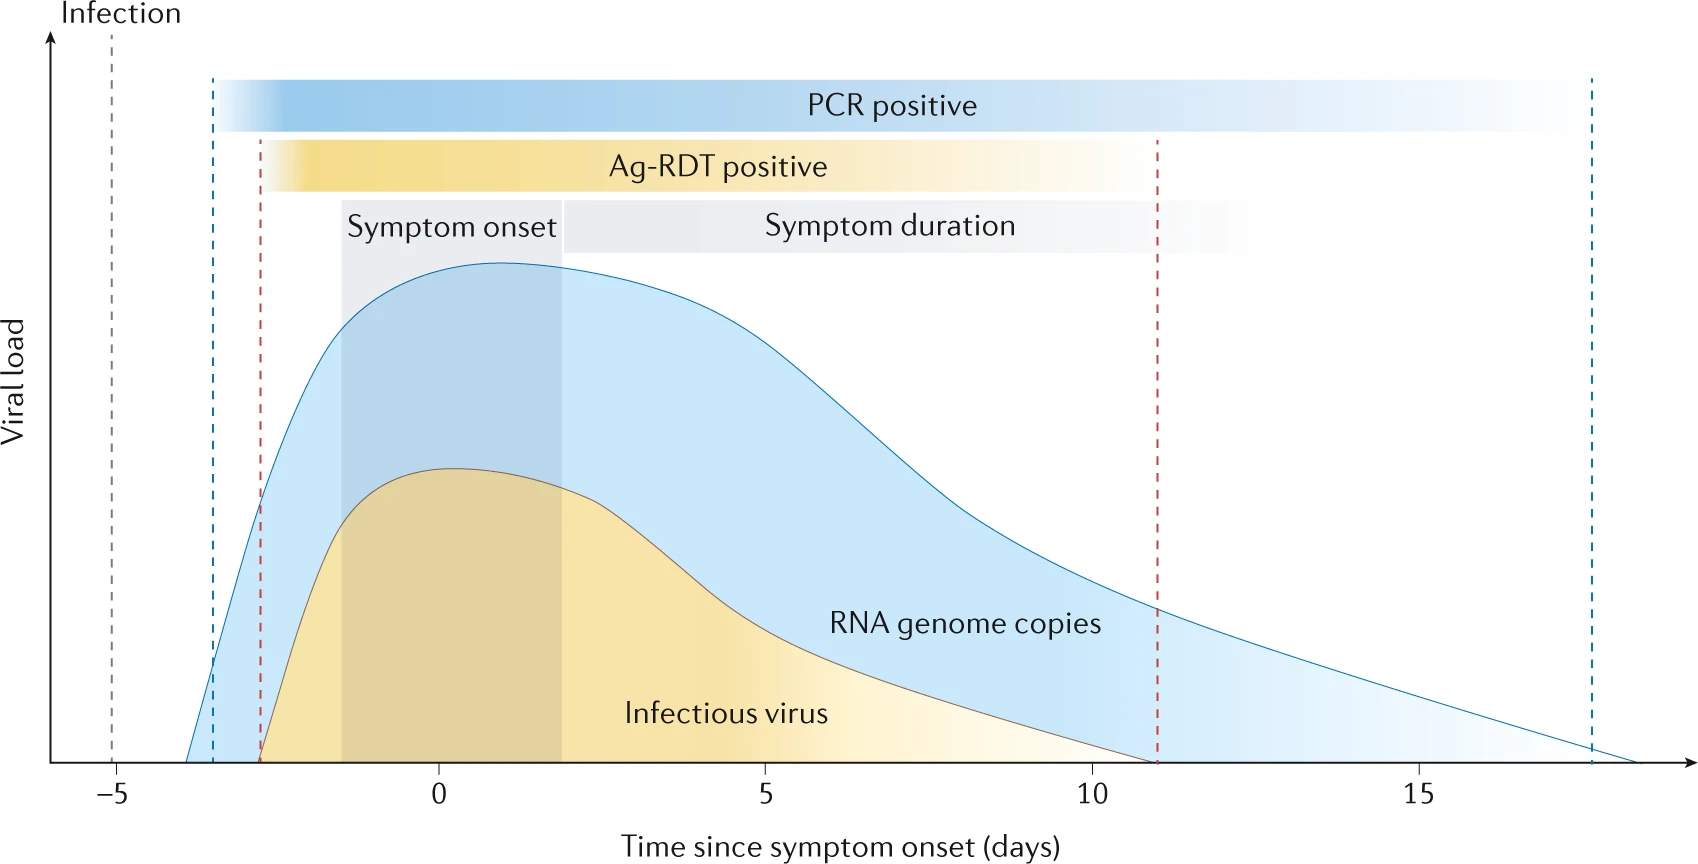
\includegraphics[width=\textwidth]{biology-data/natural-history}
  \caption[Natural history of SARS-CoV-2.]{Natural history of SARS-CoV-2. Reproduced from \textcite{puhachSARSCoV2} with permission.}
  \label{biology-data:fig:natural-history}
\end{figure}

Possible summaries
\begin{enumerate}
  \item \url{https://www.nature.com/articles/s41579-022-00822-w/figures/2}
  \item \url{https://www.nature.com/articles/s41576-021-00360-w/figures/1}
  \item \url{https://academic.oup.com/view-large/figure/305617142/ciaa1442_fig2.jpg}
\end{enumerate}

\begin{itemize}
  \item Phases: pre-infection positive, infectious positive, post-infectious positive, negative
  \item Relationship between different means of infected: infectious, PCR positive, symptomatic/diseased
\end{itemize}

\section{PCR testing} \label{biology-data:sec:PCR}

\emph{Describe how PCR testing works}

False negatives could occur for a variety of reasons, most commonly that an individual swabs themselves poorly and hence the concentration of virus on the swab is too low to be detected by the PCR process.
Plausibly, a variety of other reasons could also lead to a false negative such as logistical issues or mislabelling of samples.

Make sure I cover:
\begin{itemize}
  \item Relationship between Ct and viral load (and infectiousness?)
  \item Limit of detection
  \item The idea of being "detectable"? Check if/where/how I've used this concept in current version of text.
  \item 
\end{itemize}

Viral loads are infrequently measured exactly.
The most common form of data obtained is cycle threshold (Ct) values from real-time quantitative  reverse-transcriptase polymerase chain reaction (PCR) tests.
The Ct value is proportional to the negative log of the viral load which is convenient when modelling log viral load as a piecewise linear function, since Ct values themselves are piecewise linear under this assumption.
When a host's viral load is too low (below the limit of detection of the PCR test), no Ct value is available and hence viral load can be considered censored at the limit of detection.
The relationship between Ct and viral load is noisy and can vary based on many factors including quality of swab obtained, primers used (even between batches), and the PCR system set-up~\autocites{dahdouhCt,hanRTPCR}.

\section{Studies used in this thesis}

\subsection{Assessment of Transmission and Contagiousness of COVID-19 in Contacts}

\subsection{Coronavirus (COVID-19) Infection Survey} \label{intro:sec:cis}

The CIS (Coronavirus (COVID-19) Infection Survey) continually enrols individuals and tests them on an ongoing basis, following a
specified testing protocol. The protocol specifies that the initial five
tests are spaced every 7 days, then the spacing is every 28 days.
However, real-world considerations often lead to variations in test
times and missed tests. Our analysis focuses solely on the binary result
(positive or negative) of these tests, assuming no misclassification
bias.

The CIS (Coronavirus Infection Survey) is a longitudinal study on a representative sample of households.
Households are invited to the study from databases held by the ONS.
The number invited was to satisfy various target number of individuals swabbing per fortnight.
Within a selected household, all individuals aged 2 and over were invited to participate.
Once invited, an enrolment swab would be taken followed by 4 further weekly swabs (giving a total of 5 swabs on days 0, 7, 14, 21, 28 relative to enrolment) after which monthly swabs are taken.
A full description of the study can be found in \textcite[][supplementary materials]{pouwelsCommunity} or the study protocol~\autocite{cisProtocol}.

During the period we consider, the total cohort size expands due to the continuous recruitment into the study.
Following this, the number then decreases and stabilises as those recruited to meet the October target transition from weekly onto monthly testing.

\todo[inline]{Add some descriptive figures e.g. those in \url{~/COVID/ons-incidence/duration_estimation/reproducible-sims/reports/simulation-studies.pdf}}

Consider the CIS data.
It consists of a series of tests on the same individuals (longitudinal data), where some individuals have a series of positive tests.

\subsubsection{Episodes}

\emph{Explain definition in ``SARS-CoV-2 reinfection definition'' from \textcite{weiRisk}.}

\emph{Intermittent negatives} are the clearest example of a false negative.
An intermittent negative is when an individual tests negative but tested positive previously and subsequently.
Intermittent negatives are stripped out when creating the dataset used for all duration analyses in this chapter, but demonstrate that false negatives do occur.

% Whether a future positive is part of the same episode of a reinfection is not always trivial; I rely on a process developed previously by Sarah Walker, see \cref{E-episode-def}.
However, up until the emergence of the Omicron variant, reinfections are rare, especially in a short time frame, and hence the tricky cases are rare until this time (late 2021).


\ifSubfilesClassLoaded{
  \listoftodos
}{}

\end{document}